\documentclass[border=10pt]{standalone}
\usepackage[european]{circuitikz}
\begin{document}
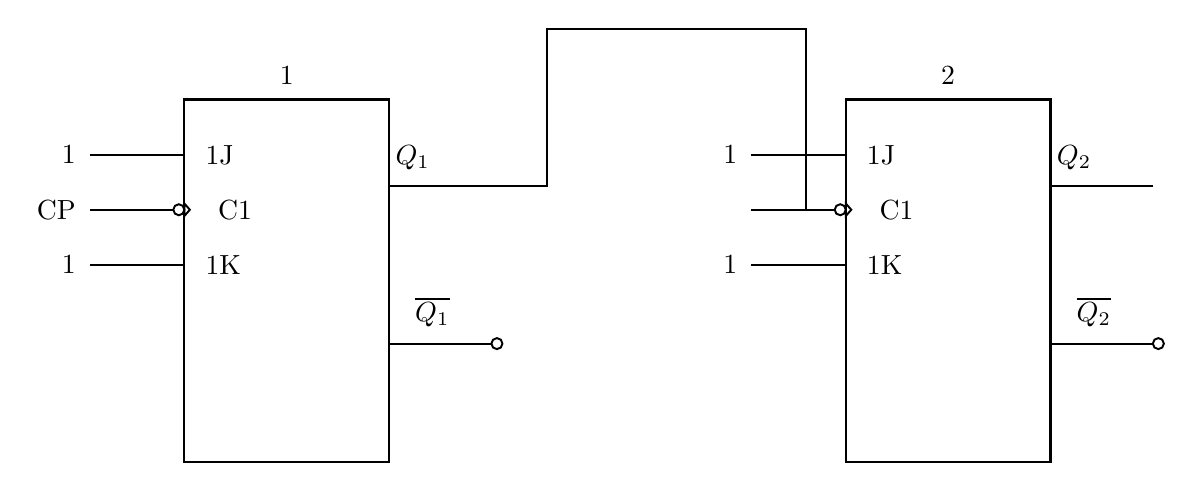
\begin{tikzpicture}[line width=0.7pt, font=\normalsize]

% 图 8.06：两级 JK 级联（J=K=1，下降沿；第二级 C1 ← 第一级 Q1，CP 只接第一级）
% 数据照课程站 2026-10-28 页转写表，不自行补条件。
% 框 2.6 x 4.6；输入行 3.9 / 3.2 / 2.5；Sbar/Rbar 本题不画（页面转写表无此行）
% 通道：Q1 → 第二级 C1 走顶部 y=5.5；两级 1 输入各自左侧短引线。

\newcommand{\jk}[2]{% #1 x  #2 级号
  \begin{scope}[shift={(#1,0)}]
    \draw[thick] (0,0) rectangle (2.6,4.6);
    \node[anchor=south] at (1.3,4.66) {#2};
    \node[anchor=west] at (0.14,3.9) {1J};
    \draw (0,3.9) -- (-1.2,3.9);
    \node[anchor=east] at (-1.25,3.9) {1};
    % 时钟端：下降沿（三角内缩 + 外圈）
    \node[anchor=west] at (0.3,3.2) {C1};
    \draw (0,3.12) -- (0,3.28) -- (0.07,3.2) -- cycle;
    \draw (-0.07,3.2) circle (0.07);
    \draw (-0.14,3.2) -- (-1.2,3.2);
    \node[anchor=west] at (0.14,2.5) {1K};
    \draw (0,2.5) -- (-1.2,2.5);
    \node[anchor=east] at (-1.25,2.5) {1};
    \draw (2.6,3.5) -- (3.9,3.5);
    \node[anchor=south] at (2.9,3.58) {$Q_{#2}$};
    \draw (2.6,1.5) -- (3.9,1.5);
    \draw (3.97,1.5) circle (0.07);
    \node[anchor=south] at (3.15,1.58) {$\overline{Q_{#2}}$};
  \end{scope}
}

\jk{0}{1}
\jk{8.4}{2}

% CP 只接第一级
\node[anchor=east] at (-1.25,3.2) {CP};

% Q1 → 第二级 C1（顶部通道；终点高度 3.2）
\draw (3.9,3.5) -- (4.6,3.5) -- (4.6,5.5) -- (7.9,5.5) -- (7.9,3.2) -- (8.25,3.2);
% Qbar1 引出但不接（本级悬空输出，页面转写表只要求 Qbar 存在）
\node[anchor=south] at (11.05,4.02) {};
\end{tikzpicture}
\end{document}
